\chapter{Software Architecture}
\section*{12 - Ottobre}
\textbf{Architecture} is the fundamental organization of a software system embodied in its \textit{components} their relationships to each other and to the environment,
and the principles guiding its design and evolution.

\section{Component}
A \textbf{component} is the element of implementing a coherent set of features;
it can be seen as a collection of services,
possibly used by other components, 
either directly or through an API.


Architectural design issues
\begin{itemize}
    \item Non-functional product characteristics: security, reliability, availability...
    These aspects are as important as functional properties, to develop a successful product.
    \item Product lifetime:
    in case of developing a hopefully long-term product,
    its architecture must be able to evolve and adapt:
    \textit{microservices}, for instance, easily allow scalability increasing the lifetime of our product.
    \item Software compatibility:
    Usually there may be legacy modules in the system,
    thus compatibility may be crucial,
    and it may lead to limiting architectural choices.
    \item Number of users:
    Releasing software on the internet truly complicates the prediction of the number of users for a product,
    it may vary a lot,
    thus the architecture must allow scaling up and down according to it.
    \item Software reuse:
    reusing components from other products or open-source software might save a lot of \textit{time} and \textit{effort},
    however it may force some architectural design choices.
\end{itemize}

\section{Non-functional quality attributes}
\begin{enumerate}
    \item Responsiveness \textit{Does the system return results in reasonable time?}
    \item Reliability \textit{Do features behave as expected?}
    \item Availability \textit{Can the system deliver services when requested by the users?}
    \item Security \textit{Does the system protect itself and user data from attacks and intrusions?}
    \item Usability \textit{Are the users able to access (quickly) the features they need?}
    \item Maintainability \textit{Can the system be easily updated with undue costs?}
    \item Resilience \textit{Can the system recover in case of failure or intrusion?}
\end{enumerate}
This typically aren't \textit{\st{features}} \textit{attributes} (?) implemented in the mid-development \textbf{prototypes},
they usually refer to the \textbf{final product}.
Implementing these in the prototypes would increase too much the time taken to develop such prototypes.
\nl
Besides, note that optimizing one non-functional attribute might affect others,
so, depending on our product and our resources,
it must be considered whether to focus on one attribute instead of another one.
\[
    \color{OliveGreen}
    \begin{array}[pos]{ccc}
        \textit{Security} & \xrightleftharpoons{\hspace*{3cm}} &
        \begin{array}{c}
            \textit{Performance} \\
            \textit{Usability}
        \end{array}
    \end{array}
\]
\[
    \color{mauve}
    \begin{array}[pos]{ccc}
        \textit{Availability} & \xrightleftharpoons{\hspace*{3cm}} &
        \begin{array}{c}
            \textit{Time-to-Market} \\
            \textit{Simplicity}
        \end{array}
    \end{array}
    % }
\]


\subsection{Maintainability}
For example let's consider which design choices would improve \textit{maintainability}.
First, recall that indicates how difficult and expensive is to make changes after the product release.\\
Two good practies are \textbf{decompose} the system into small self-containing parts and to avoid \textbf{shared data-structures}.\\
Speaking of \textit{shared data-structures},
a shared and \textit{centralized} DB, might act as a bottleneck or, even-worse,
as a single point of failure.\\
Using smaller local DBs for each \textbf{component} which later synchronize with the main one would avoid these two issues,
however it introduces the need for \textbf{consistency} techniques and rules.
\begin{figure}[h]
    \centering
    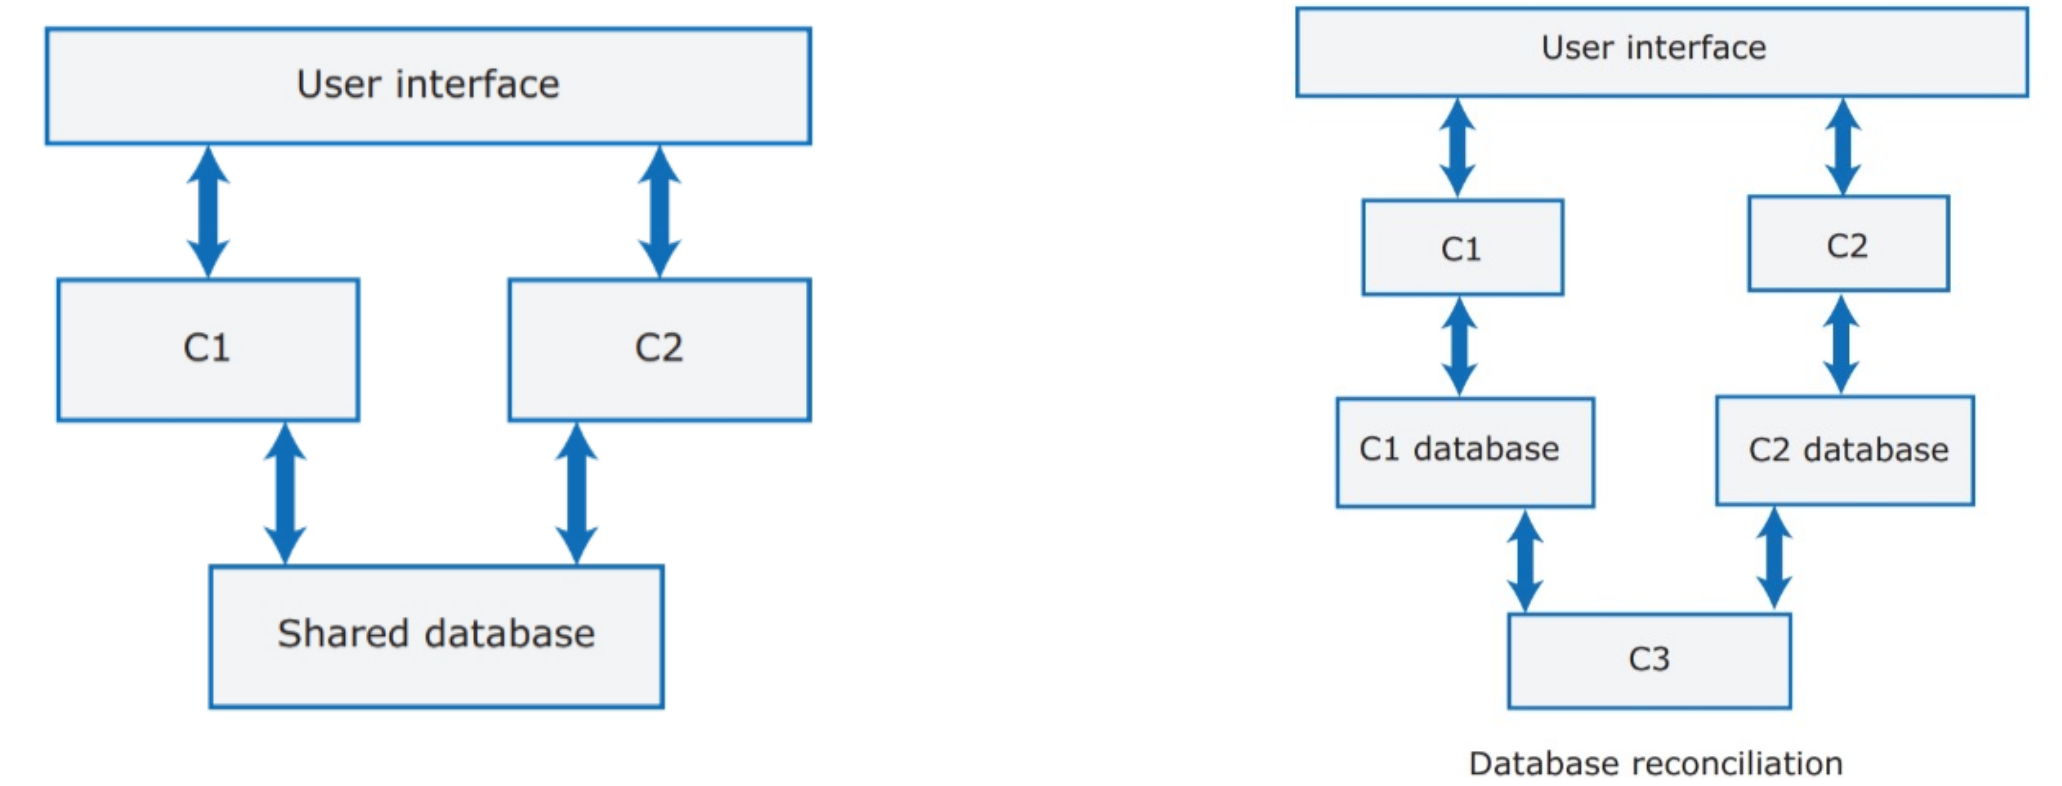
\includegraphics[width=0.7\textwidth]{images/component_DBs.png}
    \caption{Centralized vs Component DBs}
\end{figure}

\subsection{System Decomposition}
Let's dig in deeper into system decomposition, by first introducing some definitions:
\begin{itemize}
    \item \textbf{Service}: coherent unit of functionality
    \item \textbf{Component}: software unit offering one or more services
    \item \textbf{Module}: set of components
\end{itemize}
The agile manifesto suggests that: \textit{Simplicity is essential};
regarding decomposition this is particularly true since as the number of components increases,
the number of relationships betweeen them increases at a faster rate,
thus it necessary to \textbf{manage complexity};
there are a few techniques to do so:
\begin{itemize}
    \item \textbf{Separation of concerns}
    \item \textbf{Stable interfaces}
    \item \textbf{Implement once}
\end{itemize}

One way to implement this is to have a \textbf{layered architecture} where to each \textit{layer} corresponds a \textit{concern}, and the components within the same layer are independent and do not overlap in functionality.
\begin{figure}[h]
    \label{fig:layered_architecture}
    \centering
    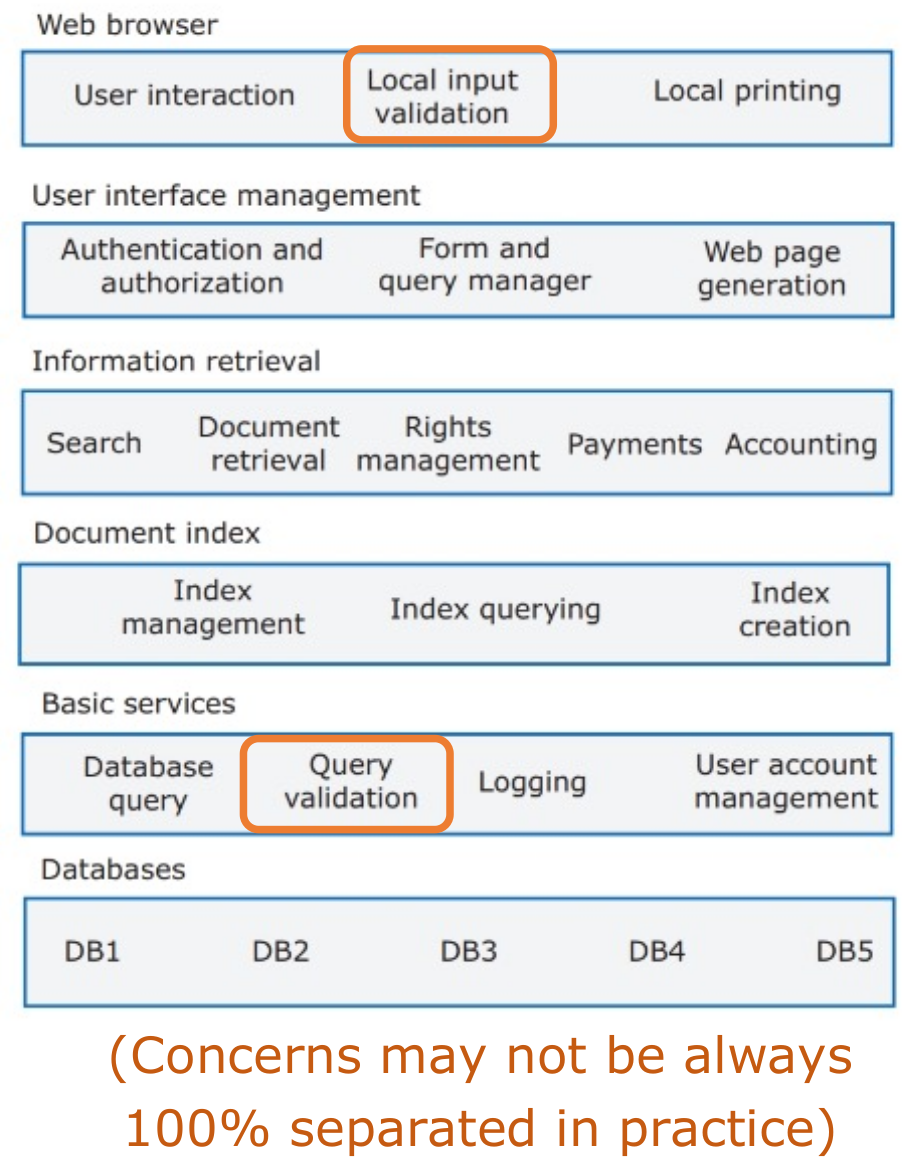
\includegraphics[width=0.45\textwidth]{images/layered_architecture.png}
    \caption{Layered architecture}
\end{figure}
There are also some "concerns", which are in fact non-functional attributes like \textit{security, performance} and \textit{reliability}, which are \textit{"cross-cutting"} i.e. they affect the whole system in a "vertical way" (see Fig \ref{fig:layered_architecture}) and they define the interaction between layers.


System decomposition must be done in conjunction with choosing technologies for the system.
In this there is a mixup happening between implementation and design, however it is necessary.
For example, the choice of a particular type of DB affects components at higher levels, or choosing to support interfaces on mobile devices implies the need for mobile UI toolkits.

\section{Distribution architecture}
Now, how can we define servers and the allocation of components to servers?

A very common way is  the \textbf{Client-Server architecture}
aka Model-View controller where usually the communication between client and server happens with HTTP along with JSON (/XML).
Client requests to a server are then muxed on many slave nodes which elaborate the requests.

There are some choices which must be made when designing the distribution architecture:
\begin{itemize}
    \item \textbf{Data type and Data Updates}: whether the data should be centralized or spread around and later on synchronized.
    \item \textbf{Change frequency}: if frequent changes are foreseen it is advisable to isolate components as separate services to allow easy and uncostful changes
    \item \textbf{System execution platform}: the service being accessed over the internet or being a business system, leads to consistently different design architecture.
\end{itemize}

\section{Technologies choices}
It is difficult and costful to change technologies mid-development,
thus it is important to the adequate considerations in advance and choose them properly.
Let's consider first which aspects of the architecture are strongly technology-related:
\begin{itemize}
    \item \textbf{Database} SQL $\xleftrightarrow{\hspace*{1em}?\hspace*{1em}}$ noSQL
    \item \textbf{Platform} Mobile app $\xleftrightarrow{\hspace*{1em}?\hspace*{1em}}$ web platform
    \item \textbf{Server} Dedicated in-house servers $\xleftrightarrow{\hspace*{1em}?\hspace*{1em}}$ cloud
    \item \textbf{Open-source} Any suitable \textit{open-source} solutions to be incorporated?
    \item \textbf{Development tools} Any limitations on the architecture imposed by the chosen development tools?
\end{itemize}